\documentclass[nooutcomes]{ximera}
%% handout
%% space
%% newpage
%% numbers
%% nooutcomes

%I added the commands here so that I would't have to keep looking them up
%\newcommand{\RR}{\mathbb R}
%\renewcommand{\d}{\,d}
%\newcommand{\dd}[2][]{\frac{d #1}{d #2}}
%\renewcommand{\l}{\ell}
%\newcommand{\ddx}{\frac{d}{dx}}
%\everymath{\displaystyle}
%\newcommand{\dfn}{\textbf}
%\newcommand{\eval}[1]{\bigg[ #1 \bigg]}

%\begin{image}
%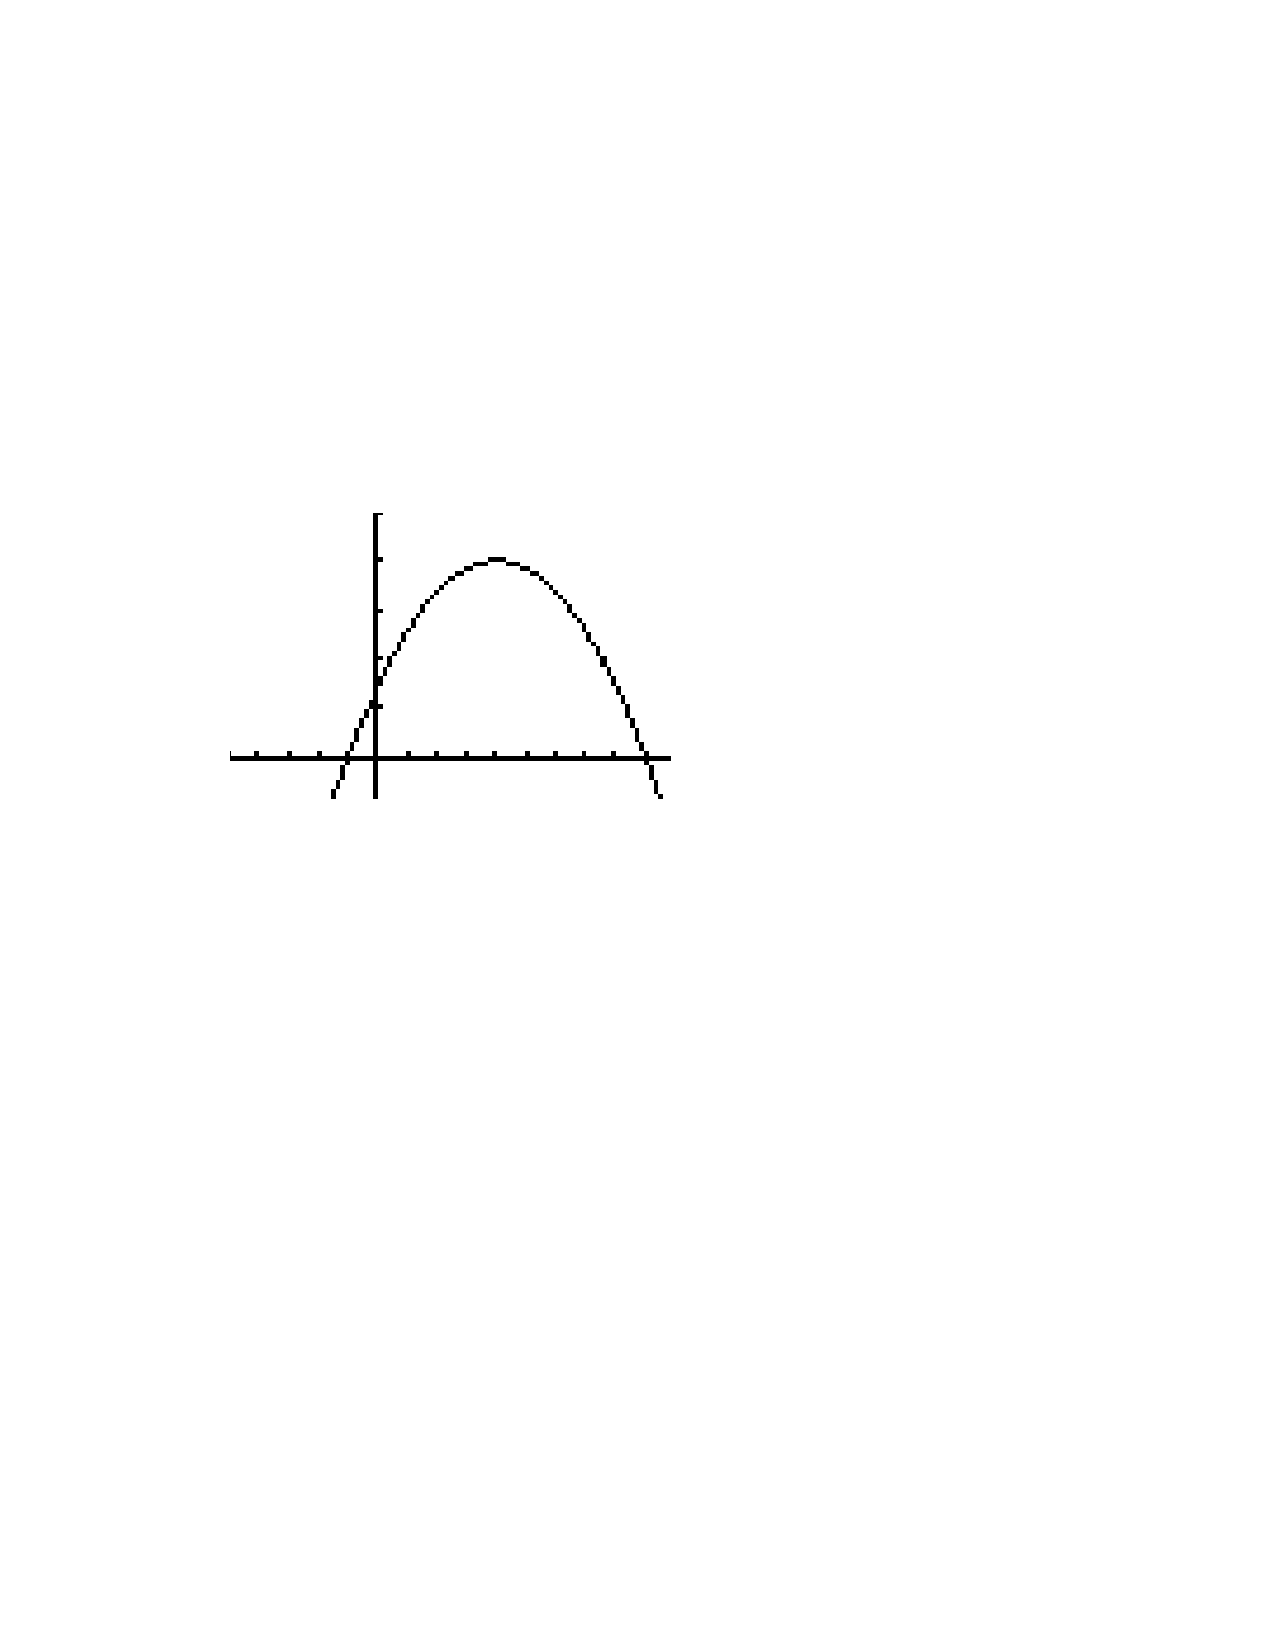
\includegraphics[trim= 170 420 250 180]{Figure1.pdf}
%\end{image}


\newcommand{\RR}{\mathbb R}
\renewcommand{\d}{\,d}
\newcommand{\dd}[2][]{\frac{d #1}{d #2}}
\renewcommand{\l}{\ell}
\newcommand{\ddx}{\frac{d}{dx}}
\newcommand{\dfn}{\textbf}
\newcommand{\eval}[1]{\bigg[ #1 \bigg]}

\usepackage{multicol}

\renewenvironment{freeResponse}{
\ifhandout\setbox0\vbox\bgroup\else
\begin{trivlist}\item[\hskip \labelsep\bfseries Solution:\hspace{2ex}]
\fi}
{\ifhandout\egroup\else
\end{trivlist}
\fi} %% we can turn off input when making a master document

\title{3.11 Related Rates}  

\begin{document}
\begin{abstract}		\end{abstract}
\maketitle


%problem1
\begin{problem}
The radius of a circle is increasing at a rate of 2 inches per minute. 
	\begin{image}
	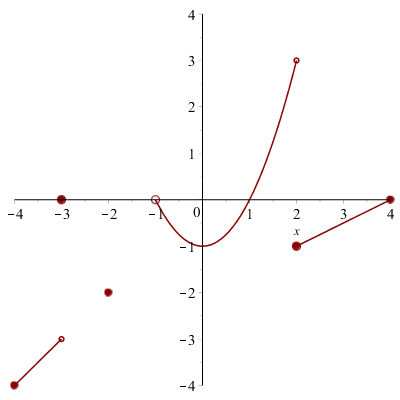
\includegraphics[scale=.5]{Figure2.png}
	\end{image}

\begin{enumerate}
	\item At what rate is the circumference of the circle changing when the radius is 10 inches?
	\begin{freeResponse}
	We know: ${\frac{dr}{dt}}=2$ inches per minute, $r=10$, and we want to find ${\frac{dc}{dt}}$.\\\\
	\begin{align*}
	c&=2\pi r\\
	{\frac{dc}{dt}}&=2\pi {\frac{dr}{dt}}\\
	{\frac{dc}{dt}}&=2 \pi (2)\\
	{\frac{dc}{dt}}&=4 \pi\ \text{inches per minute}
	\end{align*}
	\end{freeResponse}
	\item At what rate is the area of the circle changing when the radius is 12 inches?
		\begin{freeResponse}
	We know: ${\frac{dr}{dt}}=2$ inches per minute, $r=12$, and we want to find ${\frac{dA}{dt}}$.\\\\
	\begin{align*}
	A&=\pi r^2\\
	{\frac{dA}{dt}}&=2\pi r{\frac{dr}{dt}}\\
	{\frac{dA}{dt}}&=2 \pi (12)(2)\\
	{\frac{dA}{dt}}&=48 \pi\ \text{inches squared per minute}
	\end{align*}
	\end{freeResponse}
\end{enumerate}

\end{problem}




%problem2
\begin{problem}
Find the mistake in the solution to the given problem.  Then solve the problem correctly.

Two boats leave from the same dock, but at slightly different times.  One boat is traveling east at 30mph while the other boat is traveling north at 15mph.  At an instant in time when the boat traveling east is 15 miles from the dock and the boat traveling north is 10 miles away from the dock, what rate is the distance between the boats changing?
	\begin{image}
	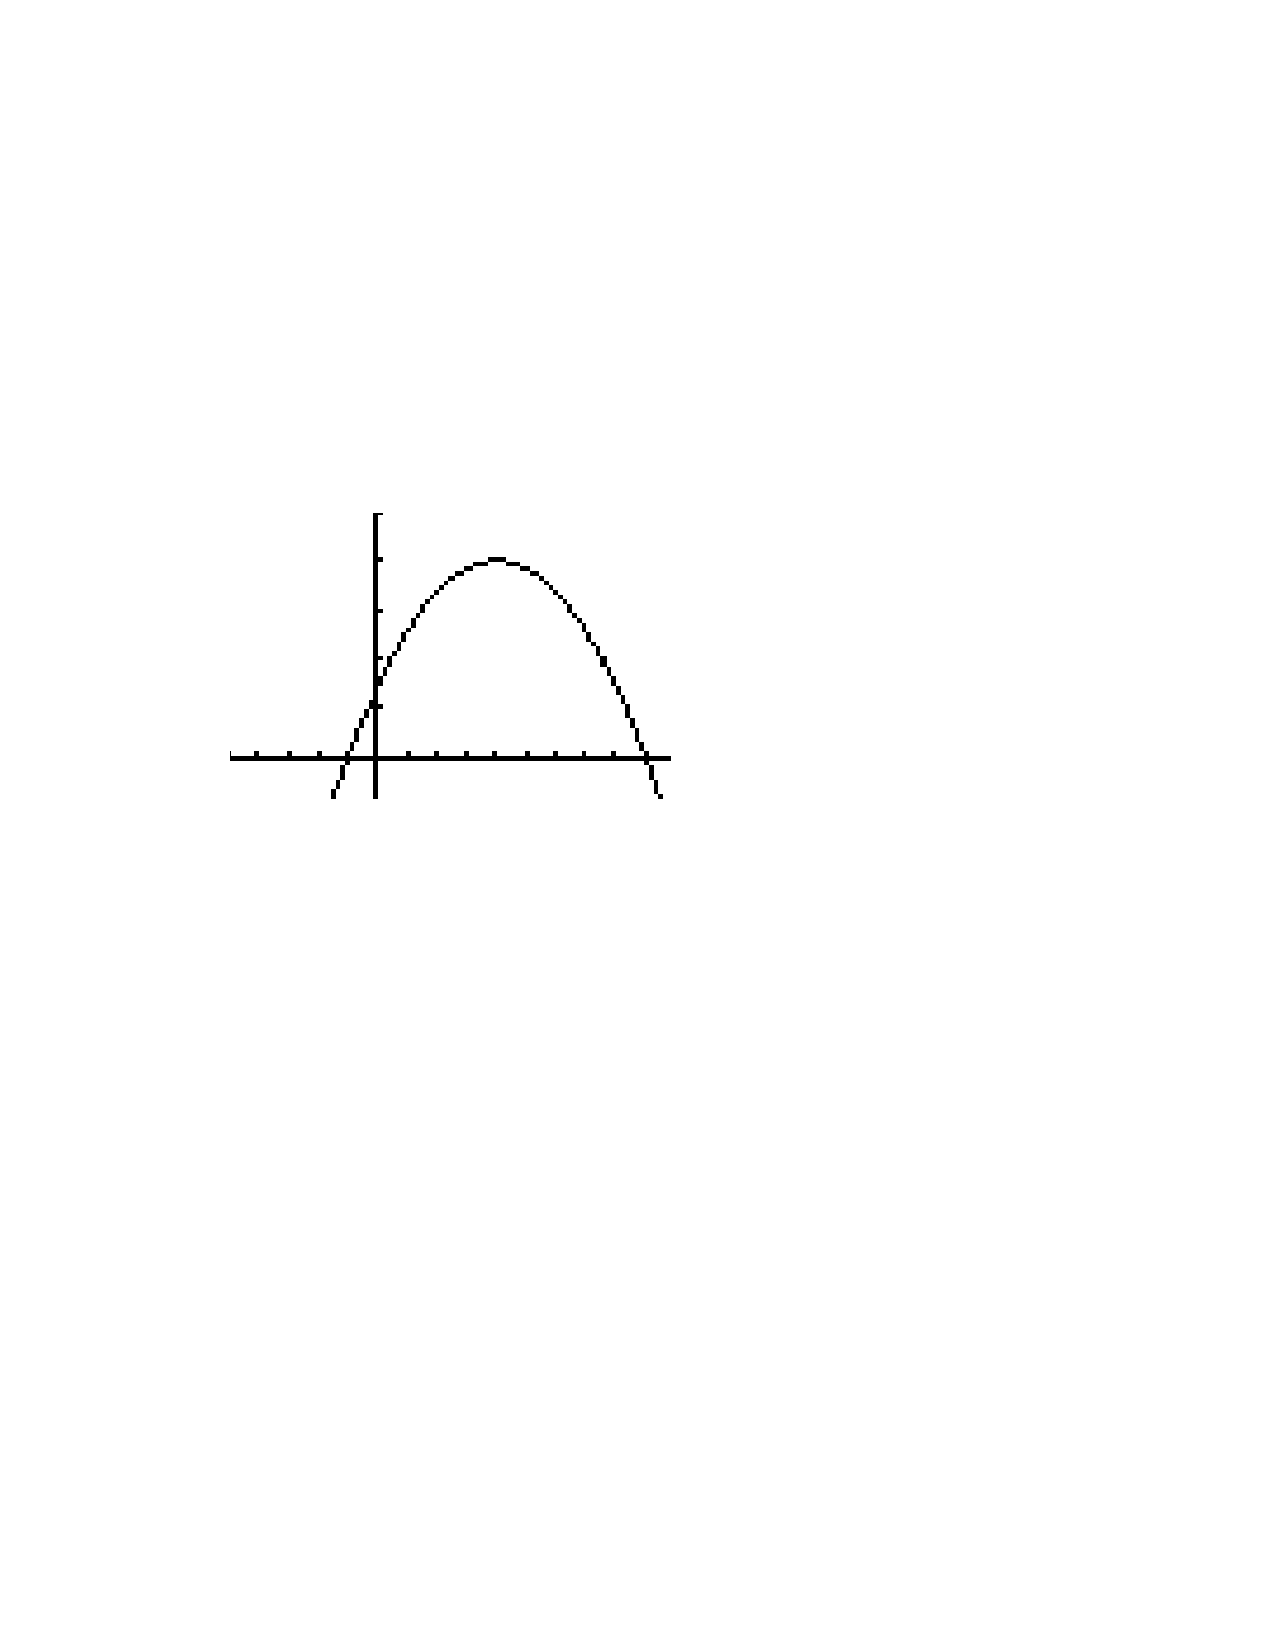
\includegraphics[scale=.7]{Figure1.png}
	\end{image}
	
		\begin{freeResponse} 
		The error occurs when the student plugs in values for $x$ and $y$ \dfn{before} differentiating the equation $x^2 + y^2 = z^2$ with respect to time.  The distances $x$ and $y$ are clearly changing with respect to time, and so they cannot be treated as constants when we are differentiating.
		
		Differentiating $x^2 + y^2 = z^2$ with respect to $t$ yields:
		$$ 2x \dd[x]{t} + 2y \dd[y]{t} = 2z \dd[z]{t}$$
		
		Canceling the 2's and plugging in the known quantities yields:
		$$ z \dd[z]{t} = (15)(30) + (10)(15) = 450 + 150 = 600 $$
		
		In the above work, the student did correctly compute that $z^2 = 325$ at this fixed instant in time.  So $z = 5\sqrt{13}$, and we can solve for $\dd[z]{t}$ to obtain
		$$ \dd[z]{t} = \frac{600}{5 \sqrt{13}} = \frac{120}{\sqrt{13}} \, mph $$
		\end{freeResponse}	

\end{problem}

%problem3
\begin{problem}
A plane flying horizontally at an altitude of 2000 m and a speed of 200 m/sec passes directly over a radar station.  (See figure below.)  Find the rate at which the distance from the plane to the station is increasing 5 seconds after the plane passed directly over the radar station.  Make sure to label the figure.

	\begin{image}
	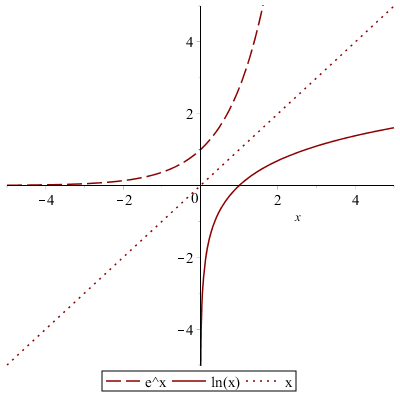
\includegraphics[scale=.5]{Figure4.png}
	\end{image}
\begin{freeResponse} \hfil

	\begin{image}
	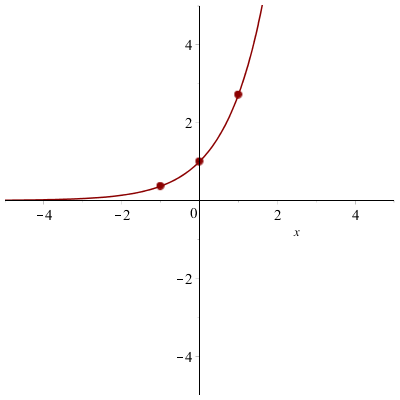
\includegraphics[scale=.5]{Figure5.png}
	\end{image}

	\begin{align*}
	y^2&=2000^2+x^2\\
	2y{\frac{dy}{dt}}&=2x{\frac{dx}{dt}}\ \text{(see $x$ and $y$ solved below)}\\
	\sqrt{1000^2+2000^2}\eval{{\frac{dy}{dt}}}_{t=5}&=1000 \cdot 200 \\
	{\frac{dy}{dt}}&=\frac{1000 \cdot 200}{\sqrt{1000^2+2000^2}}\ \text{m/s}
	\end{align*}

Solving for $x$:\\
Use $d=rt$.  Here we have $x=rt$.  $x=(5)(200)=1000$\ m  \\\\

Solving for $y$:
	\begin{image}
	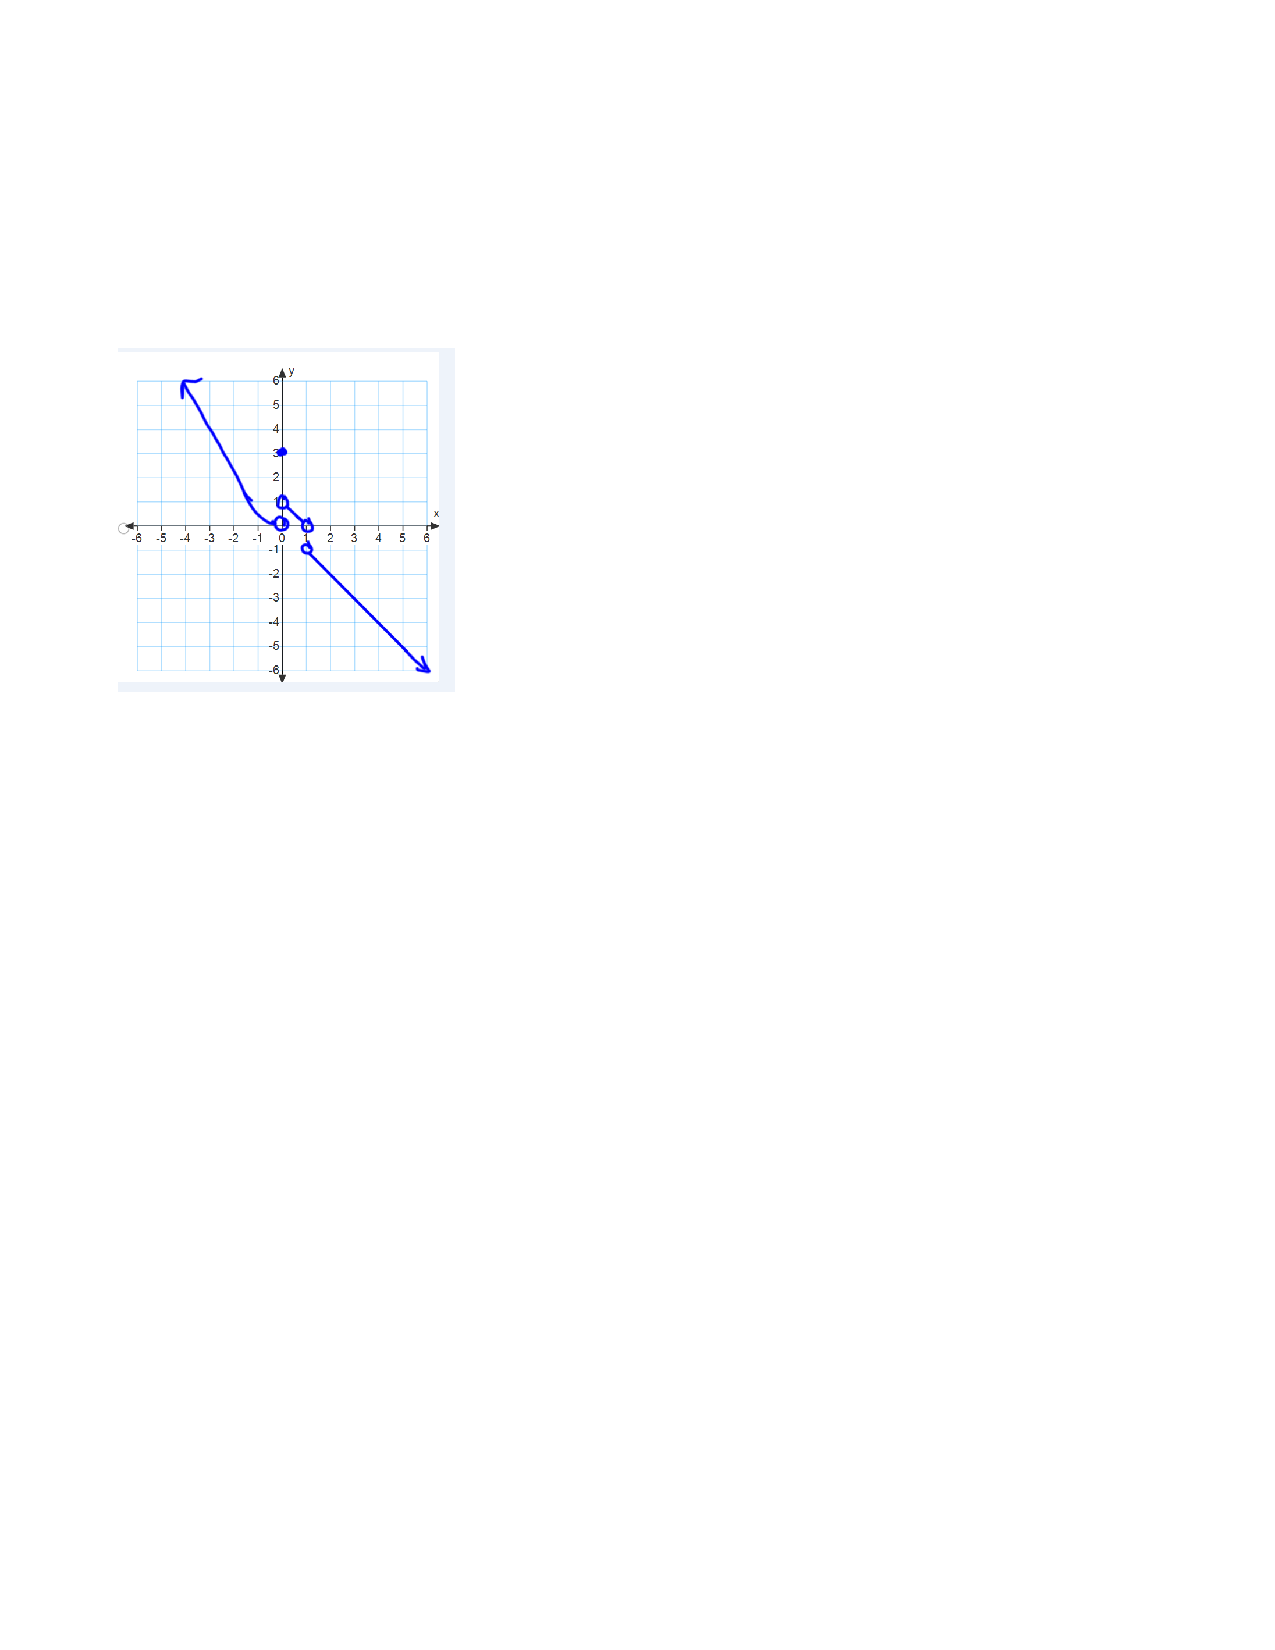
\includegraphics[scale=.5]{Figure3.png}
	\end{image}

\end{freeResponse}
\end{problem}

%problem4
\begin{problem}
A plane flying horizontally at an altitude of 800m and speed of 200 m/sec passes directly over a spectator at an air show. (See figure below.)  Find the rate at which the angle of elevation, $\theta$, is changing 4 seconds later. Make sure to label the figure. ($\theta =$\ angle between the ground and the line from the spectator to the plane)   

	\begin{image}
	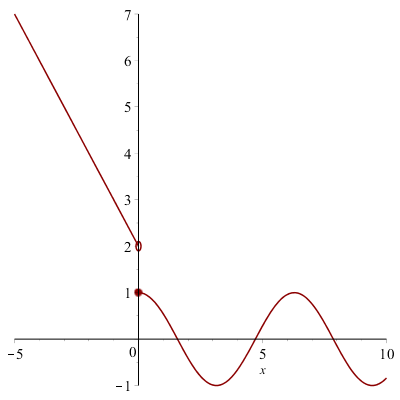
\includegraphics[scale=.5]{Figure6.png}
	\end{image}
\begin{freeResponse} \hfil
	\begin{image}
	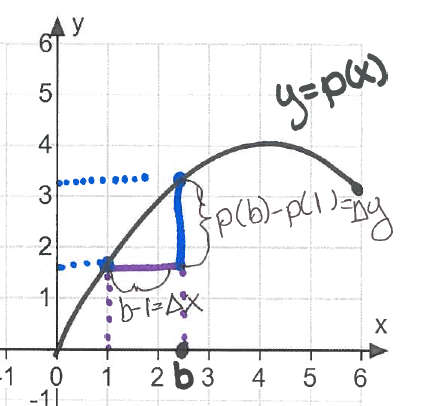
\includegraphics[scale=.5]{Figure7.png}
	\end{image}

	\begin{align*}
	\tan {\theta}&=\frac{800}{x}\\
	\sec^2{\theta} \cdot \frac{d\theta}{dt}&=\frac{-800}{x^2}\cdot \frac{dx}{dt}\ \text{(see $x$ and $\sec(\theta)$ solved below)}\\
	2 \cdot \frac{d\theta}{dt}&=\frac{-800}{800^2}\cdot 200  \\
	\frac{d\theta}{dt}&=\frac{-800}{800^2}\cdot 200 \cdot \frac{1}{2}=-\frac{1}{8} \text{radians per second}
	\end{align*}

To solve for $x$:\\
Use $d=rt$.  Here we have $x=rt$.  $x=(200)(4)=800$\ m  \\\\

To solve for $\sec{\theta}$:\\
Since the two legs of the triangle are equal, $\theta=\frac{\pi}{4}$\\
$\cos\left({\frac{\pi}{4}}\right)=\frac{1}{\sqrt{2}} \implies \sec\left({\frac{\pi}{4}}\right)=\sqrt{2}$





\end{freeResponse}
\end{problem}


%problem5
\begin{problem}
A right cone has a fixed slant height (see figure below) of 9 ft.  The cone's height is shrinking at a rate of 0.5 ft/sec.  At what rate is the area of the base changing when the height is 6 ft?  Be sure to label the picture.
	\begin{image}
	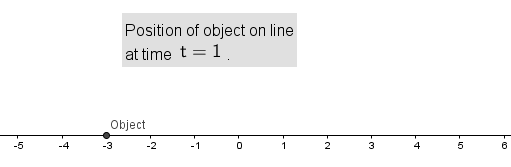
\includegraphics[scale=.5]{Figure8.png}
	\end{image}
\begin{freeResponse}
	\begin{image}
	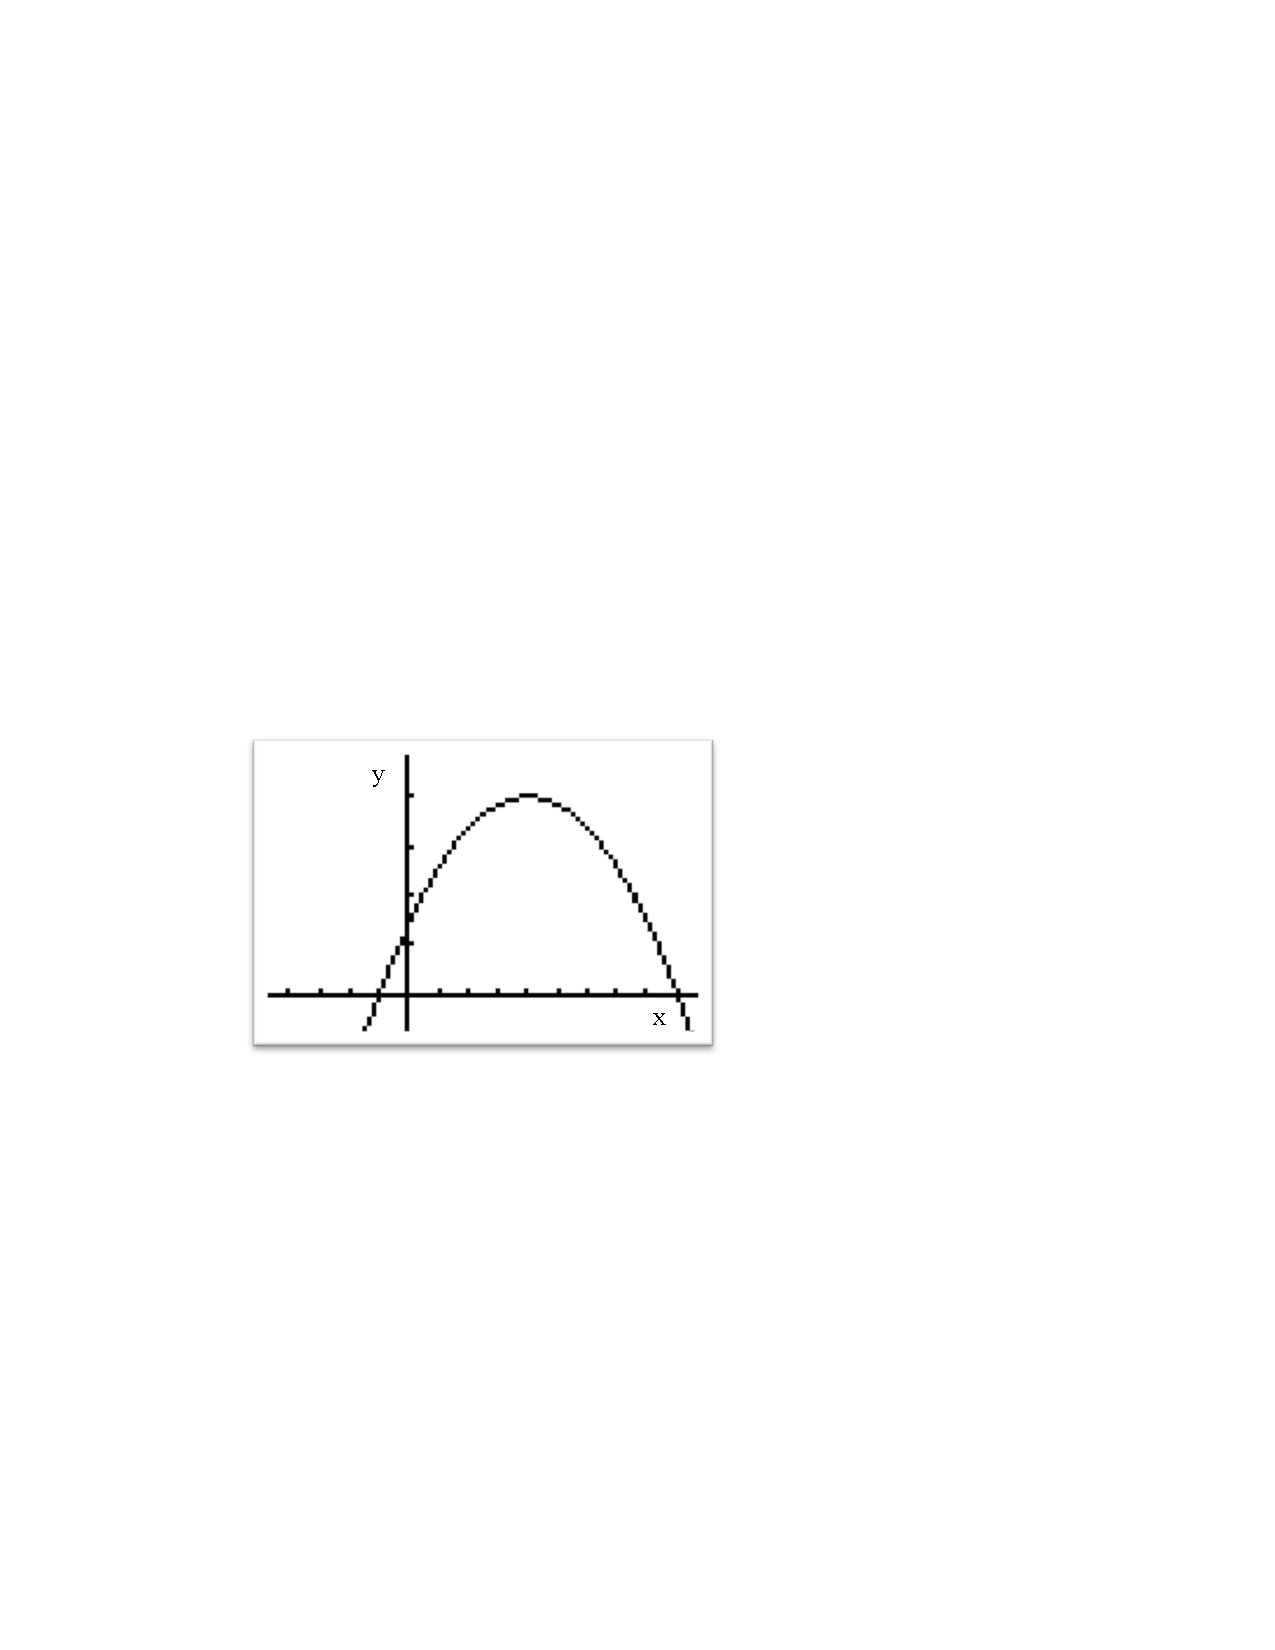
\includegraphics[scale=.5]{Figure9.png}
	\end{image}

	\begin{align*}
	A&=r^2\pi\\
	\frac{dA}{dt}&=2r\pi \cdot \frac{dr}{dt} 
	\end{align*}
	Wwe don't know $r$ or $\frac{dr}{dt}$ so we need to relate these to $h$ and $\frac{dh}{dt}$ which we do know:\\
	\begin{align*}
	r^2+h^2&=9^2\\
	2r\frac{dr}{dt}+2h\frac{dh}{dt}&=0\\
	2r\frac{dr}{dt}&=-2h\frac{dh}{dt}\\
	\text{so we have:}&\\
	\frac{dA}{dt}&=-2h\pi \cdot \frac{dh}{dt} \\
	\frac{dA}{dt}&=-2(6)\pi (-.05)\\
	\frac{dA}{dt}&=6\pi \text{feet squared per second}
	\end{align*}

\end{freeResponse}
\end{problem}

%problem6
\begin{problem}
A part of a circle centered at the origin with radius $r=7$ cm is given in the figure (A) below.  A right triangle is formed in the first quadrant (see Figure (A)).  One of its sides lies on the x-axis.  Its hypotenuse runs from the origin to a point on the circle.  The hypotenuse makes an angle $\theta$ with the x-axis.  Assume that the angle $\theta$ changes at the rate $\frac{d\theta}{dt}=0.2$\ radians per second.
	\begin{image}
	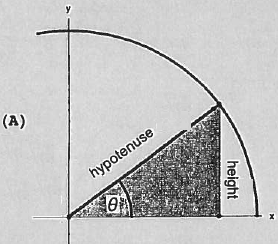
\includegraphics[scale=.5]{Figure10.png}
	\end{image}
	
\begin{enumerate}
	\item Label Figure A.
		\begin{freeResponse} \hfil
		\begin{image}
	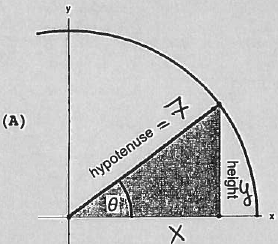
\includegraphics[scale=.5]{Figure11.png}
	\end{image}
		\end{freeResponse}
	\item In Figure B, draw the the triangle twice; one when $\theta$ is small and once more, when $\theta$ is close to $\frac{\pi}{2}$.

		\begin{image}
	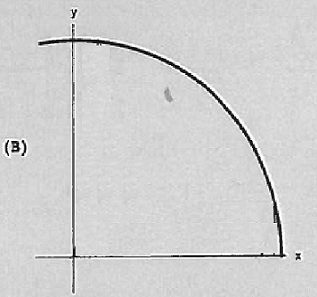
\includegraphics[scale=.4]{Figure12.png}
	\end{image}
		\begin{freeResponse} \hfil
		\begin{image}
		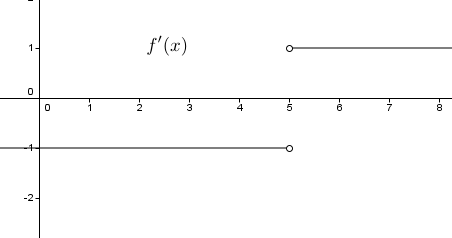
\includegraphics[scale=.5]{Figure13.png}
		\end{image}
		\end{freeResponse}
	\item Find the rate of change of the height of the triangle when $\theta=\frac{\pi}{3}$
		\begin{freeResponse}
		$y=7\sin{\theta}$
		\begin{align*}
		\frac{dy}{dt}&=\frac{dy}{d\theta}\cdot \frac{d\theta}{dt}\\
		\frac{dy}{dt}&=7\cos{\theta} \cdot \frac{d\theta}{dt}\\
		\eval{\frac{dy}{dt}}_{\theta=\frac{\pi}{3}}&=7(1/2)(0.2)\\
		&=0.7 \text{cm/sec}
		\end{align*}
				\end{freeResponse}
	\item Find the rate of change of the area of the triangle when $\theta=\frac{\pi}{3}$
		\begin{freeResponse}
		\begin{align*}
		A&=\frac{1}{2}xy\\
		A&=\frac{49}{2}\cos(\theta)\sin(\theta)\\
		\frac{dA}{dt}&=\frac{dA}{dt} \cdot \frac{d\theta}{dt}\\
		\frac{dA}{dt}&=\frac{49}{2}(-\sin^2(\theta)+\cos^2(\theta)) \cdot \frac{d\theta}{dt}\\
		\eval{\frac{dA}{dt}}_{\theta=\frac{\pi}{3}}&=\frac{49}{2}\left(-\left(\frac{\sqrt{3}}{2}\right)^2+\left(\frac{1}{2}\right)^2 \right) \cdot 0.2\\\\
		&=\frac{49}{2}\cdot \frac{1}{2} \cdot 0.2\\
		&=\frac{-4.9}{2} cm^2/sec
		\end{align*}
		\end{freeResponse}
\end{enumerate}
\end{problem}

%problem7
\begin{problem}
A floor lamp (see figure 1 below) is designed to have an adjustable height.  The lamp has a shade in the shape of a cone with radius $R=10$ inches and height $H=20$ inches.  Let $h$ be the height of the lamp.  

		\begin{image}
		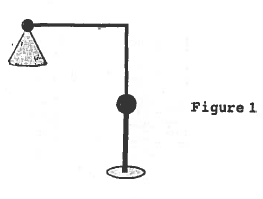
\includegraphics[scale=.5]{Figure14.png}
		\end{image}

When the lamp is on, it lights up a circular region on the floor.  (see figure 2 below).
		\begin{image}
		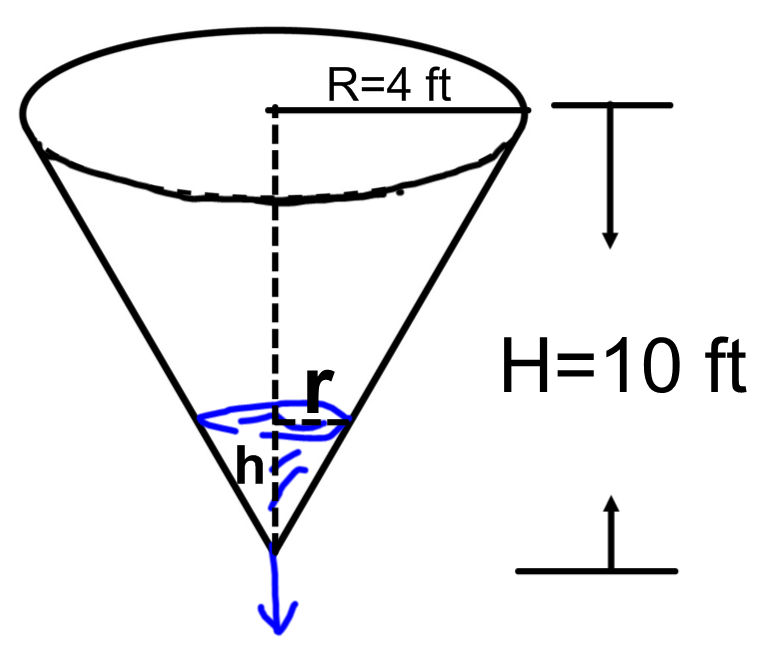
\includegraphics[scale=.5]{Figure15.png}
		\end{image}
\begin{enumerate}
	\item Let $r$ be the radiu of the lit circle.  In the figure above, lavel $r$, $R$, and $H$.
		\begin{freeResponse} \hfil
		\begin{image}
		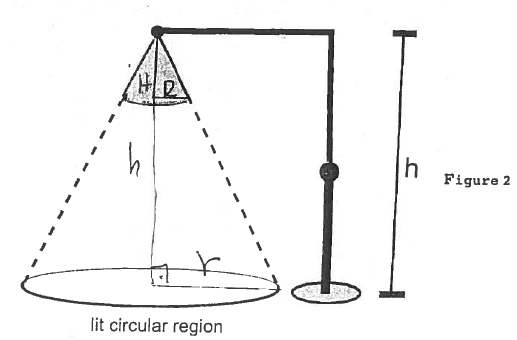
\includegraphics[scale=.5]{Figure16.png}
		\end{image}
		\end{freeResponse}	
	\item Find an expression for $r$ in terms of $h$.
	$\frac{r}{h}=\frac{R}{H}=\frac{10}{20}=\frac{1}{2}$
	
	\item Let $A$ be the area of the lit region.  Assume that the height of the lamp is decreasing at teh rate $\frac{dh}{dt}=-2$ in/sec.  Find the rate of change of $A$, the area of the lit circle, at the moment when $h=36$ inches. 
	\begin{freeResponse}
	\begin{align*}
	A&=r^2\pi\\
	\frac{dA}{dt}&=2r\pi \cdot \frac{dr}{dt} \text{see $r$ and $\frac{dr}{dt}$ solved below}\\
	\eval{\frac{dA}{dt}}_{h=36}&=36 \pi (1/2)(-2)\\
	&=-36 \pi m^2/sec
	\end{align*}

To solve for $r$:\\
$r=\frac{1}{2}h=\frac{1}{2}\cdot 36$\\\\

To solve for $\frac{dr}{dt}$:
$\frac{dr}{dt} =\frac{1}{2}\frac{dh}{dt}=(1/2)(-2)$

\end{freeResponse}
\end{enumerate}
\end{problem}

%problem8
\begin{problem}
A hot air balloon is 150 ft above the ground when a motorcycle passes directly beneath it traveling at a rate of 60 ft/sec (in a straight line on a horizontal road).  If the balloon is rising vertically at a rate of 10 ft/s, what is the rate of change of the distance between the motorcycle and the balloon 10 seconds later?
		\begin{freeResponse}
		Let $P$ denote the point on the ground directly below the hot air balloon, let $x$ denote the distance from the motorcycle to $P$, let $y$ denote the distance from the hot air balloon to $P$, and let $z$ denote the distance from the motorcycle to the hot air balloon.  The location of the motorcycle, the hot air balloon, and the point $P$ form a right triangle, and so we have that 
		\begin{equation}\label{Pythagorean}
		x^2 + y^2 = z^2.
		\end{equation}
		  We are given that $\dd[x]{t} = 60$ and $\dd[y]{t} = 10$, and the question asks us to find $\dd[z]{t}$ at time $t=10$ (meaning 10 seconds after the motorcycle passes the point $P$).  We can also easily compute that:
		$$ x(10) = 60 \cdot 10 = 600 ft $$
		$$ y(10) = 150 + (10 \cdot 10) = 250 ft $$
		$$ z(10) = \sqrt{ 600^2 + 250^2} = \sqrt{360000 + 62500} = \sqrt{422500} = 650 ft $$
		where $x(10), y(10), and $z(10) denote the values of $x$, $y$, and $z$ 10 seconds after the motorcycle passes the point $P$.  
		
		Differentiating equation \ref{Pythagorean} with respect to time, substituting, and solving for $\dd[z]{t}$ yields:
		$$ 2x \dd[x]{t} + 2y \dd[y]{t} = 2z \dd[z]{t} $$
		$$ x \dd[x]{t} + y \dd[y]{t} = z \dd[z]{t} $$
		$$ (600)(60) + (250)(10) = (650) \dd[z]{t} $$
		$$ \dd[z]{t} = \frac{36000 + 2500}{650} \frac{ft}{sec} = \frac{3850}{65} \frac{ft}{sec} = \frac{770}{13} \frac{ft}{sec} \approx 59.23 \frac{ft}{sec} $$
		
		\end{freeResponse}
					
		
\end{problem}




\end{document} 


















